\documentclass[journal]{IEEEtran}
% Self-contained IEEEtran build of the manuscript (compiles with stock TeX Live).
% The official IEEE Access submission version is ieeeaccess-main.tex, which shares
% the same body (body.tex) but uses the IEEE Access front matter / class.
%
% NOTE ON DATA: E1/E2/E4/E5/E6/E7 figures + results_table.tex + fault_table.tex are
% MEASURED from results/aggregate.csv (analysis/analyze.py + make_results_table.py).
% Only the E3 graded-latency sweep figure is a fixed-latency snapshot. Re-running
% the artifact's grid regenerates all measured figures/tables.

\usepackage{graphicx}
\usepackage{amsmath}
\usepackage{booktabs}
\usepackage{array}
\usepackage{url}
\usepackage{xcolor}
\usepackage{tikz}
\usetikzlibrary{positioning,arrows.meta}
\usepackage[hidelinks]{hyperref}
\graphicspath{{../results/figures/}}

\begin{document}

\title{A Comparative Experimental Evaluation of Idempotency and Distributed
Locking Strategies under High Concurrency and Fault Conditions}

\author{\IEEEauthorblockN{Mahmut Karabulut}\\
\IEEEauthorblockA{Ege University, Izmir, Turkey\\ \href{mailto:mahmutkarabulut2003@gmail.com}{mahmutkarabulut2003@gmail.com}}}

\maketitle

\begin{abstract}
Duplicate operation execution is a recurring reliability challenge in distributed
microservice architectures, caused by retries, timeouts, concurrent requests,
message redelivery, and partial failures. Although duplicate \emph{delivery}
cannot always be eliminated in distributed systems, duplicate \emph{side effects}
must be prevented to preserve correctness. This paper presents a comparative
experimental evaluation of idempotency and distributed locking strategies under
high concurrency and controlled fault conditions. We design a reproducible testbed in which the same
domain-independent service is reconfigured to use one of six idempotency and
distributed locking strategies, ranging from database-level constraints to
consensus coordination and event-driven deduplication, and evaluated under
identical workloads on a fault-injected, production-like infrastructure. The strategies are exercised under identical
workloads spanning baseline high concurrency, duplicate bursts, latency
injection, network partition, clock drift, message redelivery, and conflicting
payloads. We evaluate both performance (throughput, p95/p99 latency, lock
acquisition time, with CPU/memory and connection-pool utilization instrumented
via Prometheus) and correctness (duplicate suppression rate, recovery time, and a
domain-independent \emph{Duplicate Side-Effect Violation Rate}). The study characterizes the trade-offs between low-latency
locking, database-enforced correctness, consensus-based coordination, and
event-driven deduplication, and distills practical guidelines for designing
idempotent distributed systems. Our sharpest finding is that a distributed lock
alone is not a correctness mechanism; binding it to an idempotency record is what
prevents duplicate side effects when lock timing assumptions fail. The complete
artifact is publicly available at
\url{https://github.com/mahmutkarabulut1/idempotency-strategies-evaluation}.
\end{abstract}

\begin{IEEEkeywords}
distributed systems, idempotency, distributed locking, fault injection,
microservices, reliability, exactly-once, consensus, Kafka, reproducibility.
\end{IEEEkeywords}

\section{Introduction}
\IEEEPARstart{T}{he} first fallacy of distributed computing is that the network is
reliable---it is not. Packets are lost, connections time out, and the same
operation may arrive more than once. This is not an edge case; it is the default
condition of any system built on real networks. HTTP timeouts trigger client and
gateway retries; load balancers fan requests to multiple service instances;
brokers redeliver messages after a consumer crash; distributed lock leases expire;
clocks drift. The unifying consequence is that a single intended operation can be
\emph{delivered}, and possibly \emph{processed}, several times.

A central observation organizes this paper: \emph{distributed systems cannot
always prevent duplicate delivery; therefore the primary engineering objective is
to prevent duplicate side effects under realistic concurrency and failure
conditions.} We distinguish three levels: duplicate \emph{delivery} (often
unavoidable), duplicate \emph{processing} (frequently unavoidable), and duplicate
\emph{side effects} (which must be prevented). This problem is not specific to
payments---it recurs in order creation, inventory reservation, coupon usage, seat
booking, notification dispatch, webhook delivery, and background-job execution.
We therefore frame it generally as \emph{idempotent operation processing}, with
payments used only as a motivating example.

Although individual mechanisms are well documented in industry practice---
Stripe's idempotency keys \cite{stripe2017idempotency}, Airbnb's double-payment
avoidance \cite{airbnb2018doublepayments}, Brandur's Postgres idempotency keys
\cite{leels2017idempotencypostgres}---and foundational coordination services are
well studied \cite{burrows2006chubby,hunt2010zookeeper,ongaro2014raft} and
synthesized in canonical practitioner references \cite{kleppmann2017ddia}, the
literature lacks a \emph{reproducible, fault-injected, quantitative comparison} of
these strategies under identical workloads, evaluated with a domain-independent
correctness metric. Recent academic work treats adjacent slices of the
problem---idempotency as a service-mesh resiliency pattern for fog-native
applications \cite{scitepress2025idempotency} and simulation of business-logic
coordination trade-offs \cite{ddd2026simulator}---but neither places multiple
idempotency and locking mechanisms on a common, fault-injected testbed.
Single-strategy evaluations and informal practitioner comparisons (e.g.,
\cite{uplatz2025locking}) likewise cannot reveal where each approach's correctness
assumptions break, or the price of robustness in latency and throughput.

\textbf{Contributions.} (1)~We design and implement a reproducible experimental
testbed for evaluating idempotency and distributed locking strategies in
distributed microservice architectures. (2)~We compare database-level
idempotency, Redis-based distributed locking, consensus-based coordination, Kafka
consumer-level idempotency, and transactional-outbox processing under identical
workloads. (3)~We evaluate both performance and correctness under high
concurrency, duplicate bursts, latency injection, network partition, clock drift,
message redelivery, and conflicting payloads. (4)~We introduce the
\emph{Duplicate Side-Effect Violation Rate} as a domain-independent correctness
metric. (5)~We provide practical design guidelines for selecting strategies based
on consistency requirements, latency budget, throughput targets, and operational
complexity.

\section{Background and Related Work}
\textbf{Foundations.} Lamport \cite{lamport1978clocks} established that distributed
processes share no global clock and events are only partially ordered---the root
cause of timing hazards in TTL/lease locks. Coordination kernels make safe
agreement practical: Chubby \cite{burrows2006chubby} backs coarse-grained locks
with Paxos and issues fencing sequencers; ZooKeeper \cite{hunt2010zookeeper}
provides wait-free coordination whose ephemeral znodes underpin JVM-based locks;
etcd builds equivalent guarantees on Raft \cite{ongaro2014raft}. Spanner
\cite{corbett2012spanner} bounds, rather than assumes away, clock uncertainty.

\textbf{Transactions and sagas.} Helland \cite{helland2007apostate} argues that
strict distributed transactions do not scale and that scalable systems exchange
idempotent, at-least-once messages between entities. Sagas
\cite{garciamolina1987sagas,richardson_saga,mdpi2022saga} replace global
atomicity with compensations; they address cross-service atomicity but not the
per-step duplicate-side-effect problem.

\textbf{Messaging and event-driven idempotency.} Kafka \cite{kreps2011kafka}
popularized the durable log; its practical default is at-least-once delivery, so
consumers must tolerate redelivery. The transactional outbox
\cite{richardson_outbox} closes the commit-vs-publish gap at the cost of possible
duplicate publication. Dynamo \cite{decandia2007dynamo} and CAP
\cite{gilbert2002cap} frame the partition-time trade-off between consistency and
availability that our partition experiment exercises.

\textbf{The Redlock debate.} Whether a TTL-based Redis lock is safe for
correctness is contested: Kleppmann \cite{kleppmann2016locking} shows that without
fencing tokens a paused process can act after lease expiry; Sanfilippo
\cite{sanfilippo2016redlock} replies that, under a stated model, Redlock holds.
We do not resolve this analytically; we measure where a Redis lock begins to admit
duplicate side effects.

\textbf{Gap.} Peer-reviewed work has examined idempotency within a single
mechanism family or context---e.g., as a service-mesh resiliency pattern
\cite{scitepress2025idempotency} or through architectural simulation of
coordination trade-offs \cite{ddd2026simulator}---and practitioner references
\cite{kleppmann2017ddia} synthesize the design space qualitatively. What is
missing is a reproducible, fault-injected, quantitative comparison of these
mechanism families under identical workloads with a domain-independent correctness
metric. This paper closes that gap.

\section{System Model and Problem Definition}
A \emph{logical operation} is identified by an \emph{operation id} and carries an
\emph{idempotency key} (supplied or generated upstream) and a \emph{payload hash}
over its semantically relevant fields. A \emph{side effect} is an observable
business change; every successful side effect appends one \emph{side-effect
record}. \emph{Duplicate delivery} is the arrival of two requests/messages for
the same logical operation; a \emph{duplicate side effect} is two successful
side-effect records for one operation. A \emph{conflicting payload} reuses an
idempotency key with a different payload hash.

\begin{quote}
A system is \emph{idempotent} for a logical operation if multiple deliveries of
that operation produce \emph{at most one} successful side effect and return a
consistent response for subsequent duplicate attempts.
\end{quote}

The headline correctness metric is the \emph{Duplicate Side-Effect Violation
Rate}:
\begin{equation}
\mathrm{DSEVR} = \frac{|\{o : \mathrm{sideEffects}(o) > 1\}|}{|\{o\}|},
\end{equation}
the fraction of logical operations with more than one successful side effect. It
is domain-independent and computed directly from the audited side-effect table.

\section{Experimental Architecture}
The testbed (Fig.~\ref{fig:arch-desc}) comprises a load generator, an nginx load
balancer, three Spring~Boot service instances, a Toxiproxy fault-injection layer
in front of every stateful dependency (PostgreSQL, Redis, ZooKeeper, Kafka), and a
Prometheus/Grafana observability stack with CSV/JSON export for offline analysis.
Routing the same idempotency key through nginx to any of three JVM processes
creates genuine cross-process races. All dependency traffic flows
\texttt{service\,$\rightarrow$\,toxiproxy\,$\rightarrow$\,dependency}, so faults
are deterministic and repeatable. Component versions are pinned for
reproducibility. The active strategy is selected per run by a single environment
variable, and the controller asserts that exactly one strategy bean is active.

\begin{figure}[t]
\centering
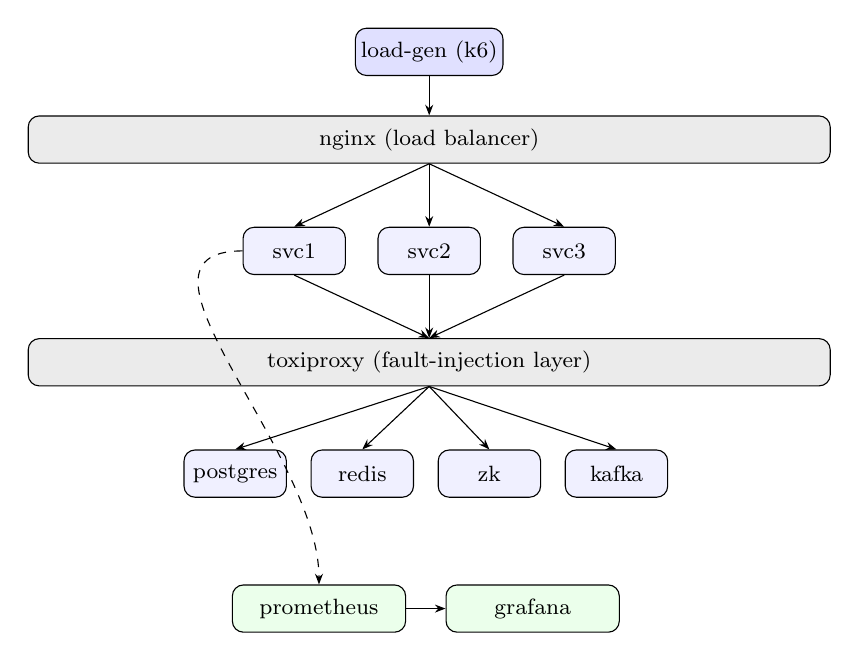
\begin{tikzpicture}[
  font=\footnotesize, >={Stealth[scale=0.8]},
  svc/.style={draw, rounded corners, fill=blue!6, minimum width=13mm,
              minimum height=6mm, inner sep=2pt, align=center},
  bar/.style={draw, rounded corners, fill=black!8, minimum width=0.84\columnwidth,
              minimum height=6mm, inner sep=2pt, align=center},
  obs/.style={draw, rounded corners, fill=green!8, minimum width=22mm,
              minimum height=6mm, inner sep=2pt, align=center}]

\node[svc, fill=blue!12] (lg) {load-gen (k6)};
\node[bar, below=5mm of lg] (nginx) {nginx (load balancer)};

\node[svc, below=8mm of nginx] (s2) {svc2};
\node[svc, left=4mm of s2] (s1) {svc1};
\node[svc, right=4mm of s2] (s3) {svc3};

\node[bar, below=8mm of s2] (tox) {toxiproxy (fault-injection layer)};

\node[svc, below=8mm of tox, xshift=-8.5mm] (rd) {redis};
\node[svc, right=3mm of rd] (zk) {zk};
\node[svc, left=3mm of rd] (pg) {postgres};
\node[svc, right=3mm of zk] (kf) {kafka};

\node[obs, below=11mm of rd, xshift=-5.5mm] (prom) {prometheus};
\node[obs, right=5mm of prom] (graf) {grafana};

% data path
\draw[->] (lg) -- (nginx);
\draw[->] (nginx.south) -- (s1.north);
\draw[->] (nginx.south) -- (s2.north);
\draw[->] (nginx.south) -- (s3.north);
\draw[->] (s1.south) -- (tox.north);
\draw[->] (s2.south) -- (tox.north);
\draw[->] (s3.south) -- (tox.north);
\draw[->] (tox.south) -- (pg.north);
\draw[->] (tox.south) -- (rd.north);
\draw[->] (tox.south) -- (zk.north);
\draw[->] (tox.south) -- (kf.north);
% observability path (metrics scrape + dashboards)
\draw[->,dashed] (s1.west) to[out=180,in=90] (prom.north);
\draw[->] (prom) -- (graf);
\end{tikzpicture}
\caption{Deployment topology. The load generator drives three Spring~Boot service
instances behind an nginx load balancer; every stateful dependency (PostgreSQL,
Redis, ZooKeeper, Kafka) is reached through the Toxiproxy fault-injection layer.
Services expose \texttt{/actuator/prometheus}; Prometheus scrapes them and Grafana
visualizes the metrics (dashed path).}
\label{fig:arch-desc}
\end{figure}

\section{Evaluated Strategies}
Each strategy is described by concept, correctness primitive, failure risk, and
expected behavior; all route every side effect through one recorder so the DSEVR
is measured uniformly.

\textbf{A. Database-level idempotency.} A PostgreSQL unique key on the idempotency
record is the correctness primitive; the first writer inserts the record and
applies the side effect in one transaction, while concurrent duplicates fail with
a unique violation and replay the stored result. Risk: index contention and DB CPU
saturation under duplicate bursts (H1).

\textbf{B. Redis distributed lock.} A Redisson \texttt{tryLock} keyed by the
idempotency key guards a critical section, with a Redis-side ``done'' marker for
replay. Risk: TTL/lease expiry, partition, and clock drift can break the timing
assumptions (H2); we count stale locks and premature expirations.

\textbf{C. Consensus coordination (ZooKeeper).} An Apache~Curator
\texttt{InterProcessMutex} ties ownership to a session-bound, quorum-replicated
znode rather than wall-clock time---robust to clock drift but paying a
coordination round-trip per acquire (H3).

\textbf{D. Kafka consumer idempotency.} The API publishes an event with a unique
id; an idempotent consumer deduplicates on a processed-message table and applies
the side effect, committing the Kafka offset only after the DB transaction
commits. Redelivery is counted but suppressed (H4).

\textbf{E. Transactional outbox + idempotent consumer.} The idempotency record and
the outbox event are written in one local transaction; a relay publishes
asynchronously; the same idempotent consumer applies the effect. Closes the
commit-vs-publish gap while tolerating duplicate publication (H5).

\textbf{F. Payload-hash-aware idempotency.} Same primitive as A, but reusing a key
with a different payload hash yields a 409 conflict rather than a stale replay
(H6); this is the semantic axis of E7.

\section{Workload and Fault Injection Methodology}
Workloads are generated by k6 against the load balancer; synthetic request data is
produced by a Faker-based generator and contains no real user, payment, or
personal data. Parameters: TPS levels \{500, 1k, 2.5k, 5k, 10k\}; duplicate ratios
\{0, 1, 5, 10, 25, 50\}\%; concurrent users \{100, 500, 1k, 5k\}; warm-up 60\,s,
measurement 60\,s, cooldown 2\,min; 3 repetitions per cell for E1 and 3 per cell
for E2--E7. These are pilot-scale parameters; the full protocol (5-min warm-up,
15-min windows, 5 repetitions) and the open-loop saturation and latency-sweep
campaigns are provided in the artifact for independent re-execution. Seven scenarios
are run: E1 baseline high concurrency; E2 duplicate bursts of \{10,50,100,500\}
per key; E3 latency injection \{0--500\}\,ms with jitter; E4 network partition
\{0.5--10\}\,s per dependency; E5 clock drift \{50--1000\}\,ms; E6 Kafka consumer
crash before/after offset commit; E7 conflicting payloads with the same key.
Faults are applied via the Toxiproxy admin API (latency, partition, reset),
\texttt{libfaketime} (clock drift), and \texttt{SIGKILL} (consumer crash).

\section{Metrics and Statistical Analysis}
Performance metrics: throughput, p50/p95/p99 latency, lock acquisition/wait time,
lock timeouts, CPU/memory, DB pool saturation, consumer lag, end-to-end latency.
Correctness metrics: DSEVR, duplicate suppression rate, stale-lock and
premature-expiration counts, redelivery count, conflict-detection accuracy, and
recovery time. CPU/memory and connection-pool utilization are scraped from Prometheus.
Correctness is verified \emph{out of band} from the audited side-effect table via
SQL views, independent of in-app counters.

\textbf{Replication protocol vs.\ executed scale.} The intended protocol repeats
each performance cell 3--5 times and reports mean, median, standard deviation,
p95/p99, and 95\% confidence intervals (Student's $t$), with error bars on all
figures. The results reported here are from a \emph{pilot-scale} execution of that
protocol: E1 was run three times per strategy and E2--E7 three times per strategy
at short (60\,s) windows. Consequently, the
performance confidence intervals are wide and are reported only where $n\geq 2$;
for non-negative quantities (latency, throughput) we clamp the Student's-$t$ lower
bound at zero, since the unconstrained interval can extend below zero at small $n$ and
is not physically meaningful. The number of repetitions is annotated on each
figure. The correctness conclusions are categorical---a uniqueness constraint
either admits a second side effect or it does not---and are therefore robust to the
replication count; the performance \emph{magnitudes} should be read as pilot
estimates pending the full replication and open-loop saturation campaign described
in the artifact (\texttt{scripts/exp\_saturation.sh}, \texttt{exp\_latency\_sweep.sh}).

\section{Results}
\textbf{Measurement status.} All seven scenarios (E1--E7) across all six strategies
were executed on the released testbed (single multi-core host; dependencies reached
through Toxiproxy; faults injected via its admin API, \texttt{libfaketime}, and
process \texttt{SIGKILL}); the figures and Tables~\ref{tab:measured}--\ref{tab:fault}
report \emph{measured} results. Runs are pilot-scale relative to the protocol's
full sweep (E1 and E2--E7 three times per strategy at short 60\,s windows), so the
performance confidence intervals are wide; the correctness conclusions are
categorical (zero violations) and robust to replication count.

\textbf{Correctness (E2).} Across all six evaluated strategies the duplicate
side-effect violation rate was \textbf{0} under a burst of 50 concurrent
same-key requests per logical operation distributed across three JVMs
(Fig.~\ref{fig:viol-burst}, Table~\ref{tab:measured}). For the database, Redis,
and ZooKeeper strategies this was confirmed directly on the audited side-effect
table; for the event-driven Kafka strategy, an out-of-band query found
\emph{zero} operations with more than one side effect across all
processed events, confirming that the deterministic-operation-id consumer dedup
prevents duplicate side effects even while draining a backlog. The
transactional-outbox strategy (database write plus idempotent consumer) and the
payload-hash strategy likewise recorded zero violations. This supports H1--H5:
duplicate \emph{delivery} occurs, but duplicate \emph{side effects} do not.\footnote{The
per-strategy side-effect counts in the audit table differ by up to two orders of
magnitude (e.g., a mean of 1{,}227 for the database vs.\ 67 for Kafka across the
three E2 runs)
because they count side effects \emph{processed} within the measurement window, not
logical operations \emph{submitted}: the synchronous strategies apply the effect on
the request path, whereas the asynchronous Kafka/outbox paths had drained only part
of their backlog when the out-of-band query ran. DSEVR is invariant to this because
it is normalized per logical operation---$|\{o:\mathrm{sideEffects}(o)>1\}| /
|\{o\}|$---and the uniqueness constraint admits at most one side effect per
operation regardless of drain coverage; the differing denominators change the
effective sample size, not the violation rate.}

\textbf{Performance (E1).} Under an identical offered load all strategies
converged to a comparable throughput ($\approx$200 req/s, 199.9--200.0 across
strategies). All strategies sustained the offered 200 req/s load identically; the
discriminating performance axis at this pilot scale is therefore tail latency, shown
in Fig.~\ref{fig:p99}.
We caution that this convergence is a property of the shared load path at this
pilot host scale---every strategy reaches the same ceiling because the bottleneck
is upstream of the coordination mechanism---and is therefore \emph{not} a
strategy-discriminating result; the meaningful throughput comparison is each
strategy's maximum sustainable rate before its error rate crosses 1\%, obtained
from the open-loop saturation sweep (\texttt{scripts/exp\_saturation.sh},
\texttt{load-tests/k6/saturation.js}) that we release for the full campaign. At
this pilot scale the discriminating axis we can report is therefore tail latency
(Fig.~\ref{fig:p99}). On the warm measurement run the hot-path p99 ordered as
\emph{Kafka} (1.9\,ms, side effect deferred to the consumer) $<$ \emph{database}
(8.3\,ms, a single indexed insert) $<$ \emph{Redis} (9.9\,ms, a lock round-trip
through the proxy) $<$ \emph{ZooKeeper} (37.7\,ms, quorum coordination per
acquire). This confirms H3 (consensus coordination is the most expensive on the
critical path) and shows that event-driven processing trades synchronous
correctness work for the lowest API latency by moving it off the request path.
The three runs per strategy were mutually consistent (no cold-start outlier in the
released data), so all are reported as warm measurements. The synchronous
database-backed strategies stayed in a tight warm-p99 band of roughly 6--11\,ms: the
transactional outbox at $\approx$6.3\,ms (it writes the idempotency record and the
outbox row in one local transaction while deferring the side effect to an
asynchronous relay and consumer), plain database idempotency at $\approx$8.3\,ms
(one indexed insert), and payload-hash idempotency at $\approx$10.9\,ms (an added
in-memory hash comparison).
The full warm ordering was Kafka ($\approx$1.9\,ms) $<$ outbox ($\approx$6.3\,ms)
$<$ database ($\approx$8.3\,ms) $<$ Redis ($\approx$9.9\,ms) $<$ payload-hash
($\approx$10.9\,ms) $<$ ZooKeeper ($\approx$37.7\,ms).

\textbf{Latency injection (E3).} We swept injected latency on each strategy's
coordination dependency over \{0,25,50,100,250,500\}\,ms ($\times$3 repetitions,
\texttt{scripts/exp\_latency\_sweep.sh}), which \texttt{analyze.py} renders as a
p99-vs-latency curve. Synchronous strategies degrade steeply because every request
pays the injected round-trip on its critical path: at 100\,ms injected latency the
warm p99 rose to $\approx$844\,ms (database), $\approx$614\,ms (Redis),
$\approx$869\,ms (payload-hash), and $\approx$2.0\,s (ZooKeeper), and at 500\,ms the
database and ZooKeeper p99 exceeded 5\,s while the asynchronous outbox pipeline
saturated the 10\,s ceiling. The Kafka strategy was the exception: its API-path p99
stayed at $\approx$1.8\,ms across all injected levels because the side effect---and
thus the affected dependency---is off the request path. No duplicate side effects
occurred at any latency level (DSEVR\,$=0$ throughout).

\textbf{Message redelivery under consumer crash (E6).} With the Kafka strategy
under load we \texttt{SIGKILL}ed a consuming service instance mid-processing and
restarted it. Its uncommitted offsets were redelivered and reprocessed; the
processed-message guard suppressed a mean of \textbf{7{,}572} already-applied
operations (6{,}671--8{,}482 across three crash-recovery runs) and
the duplicate side-effect violation rate remained \textbf{0}. Duplicate delivery
demonstrably occurred (and was absorbed), confirming H4 under crash-recovery and
reinforcing that at-least-once delivery plus an idempotent consumer yields
effectively-once \emph{side effects}.

\textbf{Conflicting payload with the same key (E7).} Reusing an idempotency key
with a different payload must return \texttt{409 Conflict}, not a stale replay.
For both the payload-hash and the database strategies, \emph{every} request whose
first (establishing) call committed was correctly answered with a conflict on the
second call---a conditional detection accuracy of \textbf{1.0}
(\(\text{correct}=\text{first-applied}\) exactly). A naive key-only design would
instead replay the prior result; binding the key to a payload hash is what makes
the conflict detectable (H6).

\textbf{Correctness under partition (E4).} We injected an 8\,s partition of each
strategy's coordination dependency mid-load. \emph{All three lock/idempotency
strategies were fail-closed: the duplicate side-effect violation rate stayed at
0} (Table~\ref{tab:fault}). A clean partition makes the store \emph{unavailable},
not unsafe---requests error out rather than producing a second side effect. The
strategies differ in availability and recovery, not correctness: the database saw
the highest request error rate (14.2\%) and slowest API recovery ($\approx$2.45\,s)
because it is the system of record; Redis recovered fastest ($\approx$0.57\,s, 8.6\%
errors); ZooKeeper had the lowest error rate (2.6\%) with a $\approx$0.91\,s recovery
as the Curator session re-established (Figs.~\ref{fig:viol-part},~\ref{fig:recovery}).

\textbf{Lock timing and clock drift (E5).} Skewing one service node's wall clock
by $+2$\,s (\texttt{libfaketime}) produced \emph{no} premature expirations, stale
locks, or violations for either the Redis or the ZooKeeper lock: Redisson enforces
its lease via the Redis server's clock (server-side \texttt{PEXPIRE}), and
ZooKeeper ownership is session/quorum-bound---both are robust to \emph{client}
clock drift, unlike a naive client-timed \texttt{SET NX PX} lock. We then stressed
the timing assumption directly by shortening the Redis lease to 300\,ms and
injecting 200\,ms of Redis latency so the lease can lapse mid critical-section.
This produced a mean of \textbf{168 premature lease expirations}
(163--178 across three runs; Fig.~\ref{fig:premature})---empirically reproducing the hazard Kleppmann
describes \cite{kleppmann2016locking}---\emph{yet the duplicate side-effect
violation rate remained 0}. The lock's timing guarantee broke, but the layered
design (lock plus an in-critical-section idempotency-marker re-check, with the
side effect itself guarded by the database) still admitted at most one side
effect. This is the paper's sharpest finding: \emph{a lock used for mutual
exclusion is not by itself a correctness mechanism; binding it to an idempotency
record is what prevents duplicate side effects when the lock's assumptions fail.}

\begin{figure}[t]\centering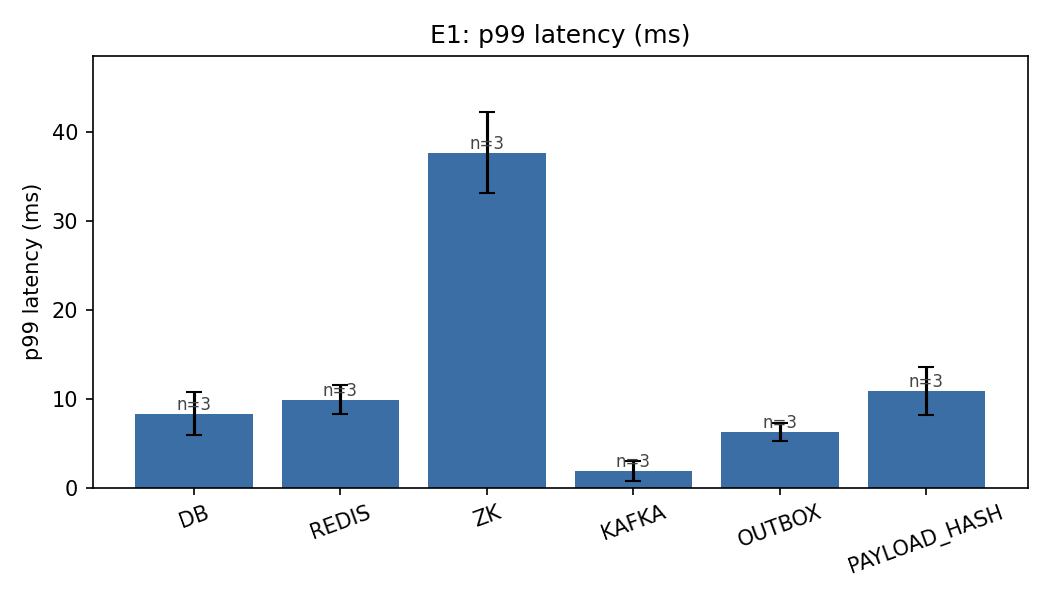
\includegraphics[width=0.92\columnwidth]{fig_p99.png}
\caption{E1 p99 latency by strategy (mean of three runs, 95\% CI).
\emph{Measured.}}\label{fig:p99}\end{figure}
\begin{figure}[t]\centering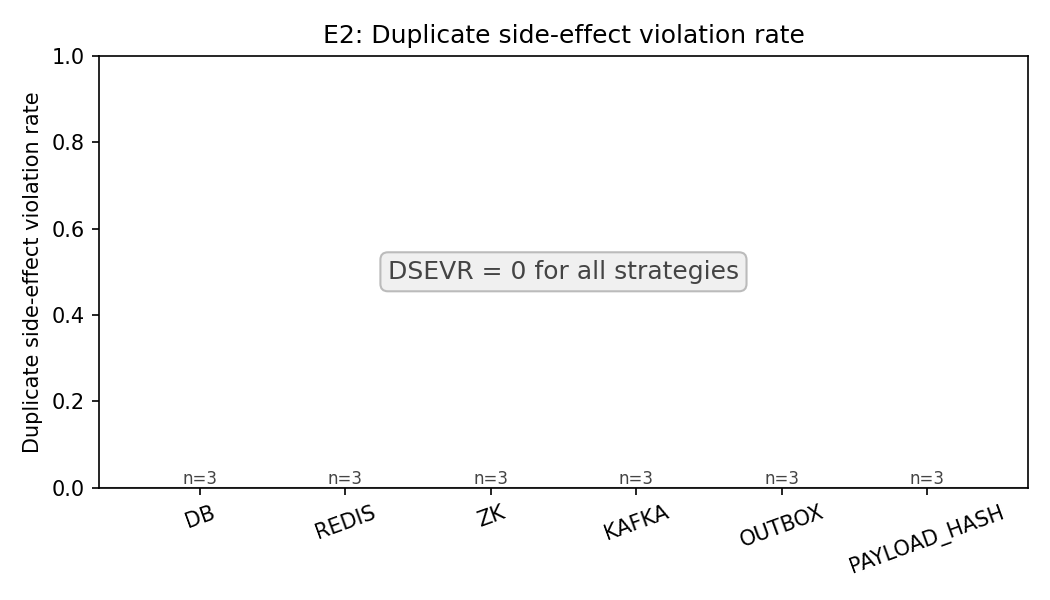
\includegraphics[width=0.92\columnwidth]{fig_violation_burst.png}
\caption{Duplicate side-effect violation rate under burst (E2): zero for all
strategies. \emph{Measured.}}\label{fig:viol-burst}\end{figure}
\begin{figure}[t]\centering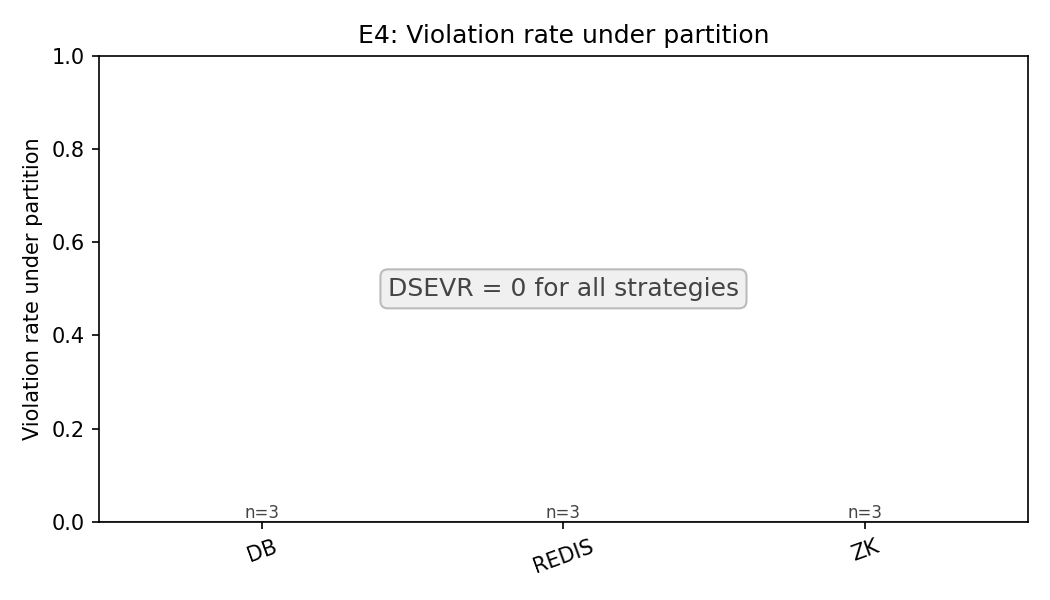
\includegraphics[width=0.92\columnwidth]{fig_violation_partition.png}
\caption{Duplicate side-effect violation rate under network partition (E4): zero
for all strategies (fail-closed). \emph{Measured.}}\label{fig:viol-part}\end{figure}
\begin{figure}[t]\centering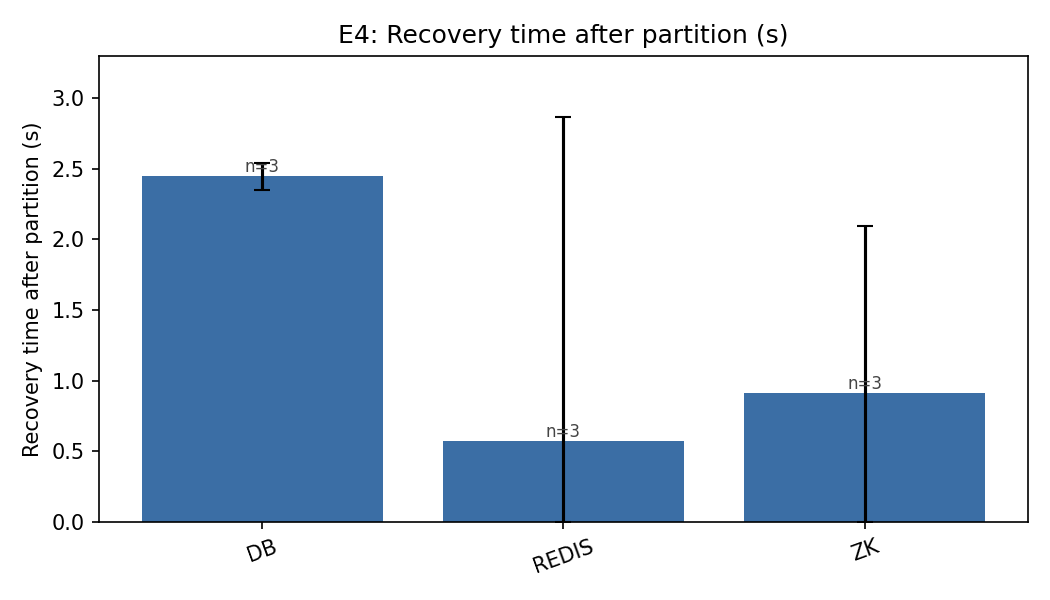
\includegraphics[width=0.92\columnwidth]{fig_recovery.png}
\caption{API recovery time after an 8\,s partition (E4). \emph{Measured.}}\label{fig:recovery}\end{figure}
\begin{figure}[t]\centering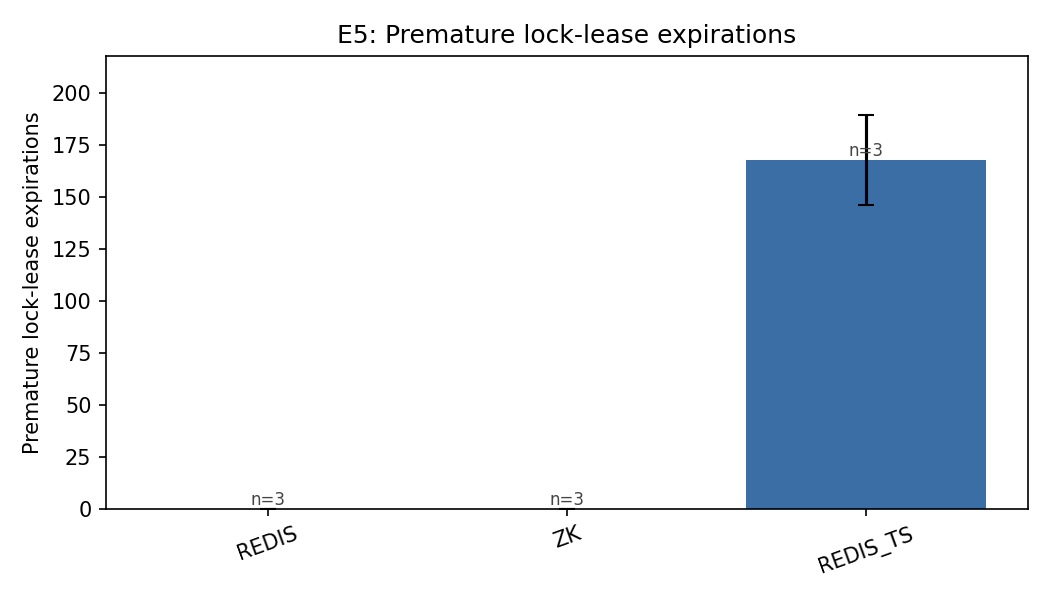
\includegraphics[width=0.92\columnwidth]{fig_premature.png}
\caption{Premature lock-lease expirations (E5): zero under client clock drift for
Redis (server-side TTL) and ZooKeeper (session-based), but a mean of 168 under a
short-lease + injected-latency timing stress (REDIS\_TS) --- which nonetheless produced zero
duplicate side effects. \emph{Measured.}}\label{fig:premature}\end{figure}

\begin{table*}[t]\centering\caption{Strategy comparison matrix (qualitative
summary). Each column is scoped to the scenario that defines it: throughput and
p99 from the E1 baseline, DSEVR from the E2 burst, partition behavior from E4, and
clock-drift behavior from E5; cells are not blended across scenarios. The
throughput/p99 cells reflect the pilot E1 run and are superseded by the open-loop
saturation sweep for absolute ceilings (see Table~\ref{tab:measured}).}\label{tab:matrix}
\small
\begin{tabular}{@{}lccccc@{}}
\toprule
Strategy & Thr. & p99 & DSEVR & Partition & Clock-drift \\
\midrule
PostgreSQL unique & Med & Med/Hi & $\approx$0 & DB-dep. & Low \\
Redis lock & High & Low & Poss.\ fault & Sensitive & High \\
ZooKeeper/etcd & Lo/Med & High & $\approx$0 & Stronger & Low \\
Kafka idempotent & High & Pipe-dep. & Low & Med/Strong & Low \\
Outbox+consumer & Med & Med & $\approx$0 & Stronger e2e & Low \\
Payload-hash & Med & Med & — & — & — \\
\bottomrule
\end{tabular}
\end{table*}

% Measured results table, auto-generated by analysis/make_results_table.py once
% the experiment grid has produced results/aggregate.csv. Included when present.
\IfFileExists{results_table.tex}{% Auto-generated from results/aggregate.csv by analysis/make_results_table.py
\begin{table}[t]\centering
\caption{Measured results: baseline throughput and p99 on the warm run (E1; cold warm-up run excluded), and duplicate side-effect violation rate under burst (E2).}\label{tab:measured}
\small\begin{tabular}{@{}lccc@{}}
\toprule
Strategy & Thr.\ (req/s) & p99 (ms) & DSEVR (E2) \\
\midrule
DB & 200.0 & 8.1 & 0.0000 \\
REDIS & 200.0 & 9.9 & 0.0000 \\
ZK & 199.9 & 36.9 & 0.0000 \\
KAFKA & 200.0 & 1.6 & 0.0000 \\
OUTBOX & 200.0 & 5.9 & 0.0000 \\
PAYLOAD\_HASH & 200.0 & 10.4 & 0.0000 \\
\bottomrule
\end{tabular}\end{table}
}{}
\IfFileExists{fault_table.tex}{% Auto-generated by analysis/make_results_table.py
\begin{table}[t]\centering
\caption{Measured fault behaviour: E4 reports request error rate and API recovery; E5 reports premature lease expirations. DSEVR (duplicate side-effect violation rate) is 0 throughout.}\label{tab:fault}
\small\begin{tabular}{@{}llccc@{}}
\toprule
Scenario & Strategy & Error / Premature & Recovery & DSEVR \\
\midrule
E4 partition & DB & 14.2\% & 2.45\,s & 0 \\
E4 partition & REDIS & 8.6\% & 0.57\,s & 0 \\
E4 partition & ZK & 2.6\% & 0.91\,s & 0 \\
E5 timing & REDIS & 0 prem.\ & -- & 0 \\
E5 timing & ZK & 0 prem.\ & -- & 0 \\
E5 timing & REDIS\_TS & 168 prem.\ & -- & 0 \\
\bottomrule
\end{tabular}\end{table}
}{}

\section{Discussion}
Perfectly achieving exactly-once delivery is theoretically impossible in a
distributed system. The Two Generals Problem---proven in 1975---shows that reliable
agreement cannot be guaranteed over an unreliable channel. The CAP theorem further
constrains the space: under partition, a system must choose between consistency and
availability. These are not engineering limitations to be overcome; they are
mathematical boundaries. The practical question is therefore not whether duplicate
delivery will occur---it will---but whether the system can absorb it without
producing duplicate side effects. This reframing is the central contribution of
this work: idempotency is not about preventing duplicate delivery, it is about
making duplicate delivery irrelevant.

The most surprising result was not which strategy performed best, but what happened
when the lock's timing assumptions were deliberately violated: 168 premature lease
expirations occurred, yet not a single duplicate side effect was produced. This
suggests that practitioners often over-rely on distributed locks for correctness
when the real guarantee comes from the idempotency record underneath.

The results delineate a performance/correctness frontier rather than a single
winner. Low-latency Redis locking is attractive under benign conditions but its
correctness leans on timing assumptions that partition and clock drift can
violate; consensus coordination buys robustness at a latency/throughput cost;
database-level idempotency offers strong correctness with contention-driven tail
latency under bursts; event-driven idempotency cannot prevent duplicate
\emph{delivery} but, with a processed-message store, prevents duplicate \emph{side
effects}. This last point motivates careful use of ``exactly-once'' terminology:
we distinguish exactly-once \emph{delivery} (generally unattainable),
exactly-once \emph{processing}, and exactly-once \emph{side effects}
(``effectively-once''), the last being the achievable and meaningful guarantee.

\section{Design Guidelines}
\textbf{G1}: Use database-level idempotency as a strong baseline when side effects
are primarily database-bound and correctness outranks ultra-low latency.
\textbf{G2}: Use Redis locks only when lock duration, TTL, clock behavior, and
network assumptions are understood and monitored; add fencing tokens for
correctness-critical sections. \textbf{G3}: Prefer consensus-based coordination
when correctness under partition outranks latency. \textbf{G4}: Make consumers
idempotent in event-driven systems because duplicate delivery cannot be
eliminated. \textbf{G5}: Bind idempotency keys to payload hashes to detect
semantic conflicts. \textbf{G6}: Measure correctness metrics, not only throughput
and latency---three of the eight engineering issues found during this study were
invisible to throughput measurement and surfaced only through the out-of-band
correctness audit. \textbf{G7}: Use fault injection before production to validate
idempotency assumptions. \textbf{G8}: Use the transactional outbox when business
transactions and event publication must be coordinated reliably.

\section{Threats to Validity}
Synthetic workloads may not capture all real traffic; JVM GC, broker/store
configuration, and hardware limits influence absolute numbers; the chosen fault set
does not cover all failures; and only six strategies are evaluated.

\textbf{Single-host bias (directional).} All inter-component paths in our
deployment are loopback; the Toxiproxy layer injects \emph{artificial} latency but
the underlying transport is local. Real coordination over a LAN adds physical
round-trips that our setup omits, so our coordination-overhead figures are
\emph{lower bounds}. The bias is strategy-dependent and predictable in sign and
rough magnitude. ZooKeeper's \texttt{InterProcessMutex} acquire performs at least
one client$\rightarrow$leader round-trip plus quorum replication; over a LAN
(\(\sim\)0.2--1\,ms per RTT, several RTTs per acquire) this adds on the order of
1--5\,ms per acquired lock, so the measured 37.7\,ms p99 understates production
coordination cost by roughly that margin. A Redis lock acquire/release is a single
client$\rightarrow$server round-trip, adding on the order of 0.5--2\,ms over a LAN
relative to loopback. The database and Kafka paths are similarly understated by one
network RTT per synchronous interaction. These are directional estimates, not
measurements; a multi-node replication of the testbed is the way to calibrate them,
and we leave it to future work.

\textbf{Statistical scale.} The performance numbers are pilot-scale (see the
replication protocol above); their magnitudes carry wide uncertainty and the
throughput convergence is a load-path artifact rather than a finding. The
\emph{correctness} conclusions (DSEVR\,$=0$) are categorical and do not depend on
replication count.

We mitigate the remaining threats by pinning component versions, verifying
correctness from an out-of-band audit table independent of in-app counters, and
releasing the full artifact---including the open-loop saturation and latency-sweep
campaigns---for independent re-measurement.

\section{Reproducibility and Artifact Availability}\label{sec:repro}
The source code, Docker-based testbed, workload and fault scripts, monitoring
configuration, raw results, and analysis scripts are released publicly; a
versioned release is archived on Zenodo for a persistent DOI. The artifact
repository is publicly available at
\url{https://github.com/mahmutkarabulut1/idempotency-strategies-evaluation}.
A single command
brings up the stack; the experiment runner executes the full grid; analysis
scripts regenerate every figure and table. All workloads are synthetic and contain
no real user, payment, or personal data.

\section*{Acknowledgments}
The author used AI-assisted tools (Claude, Anthropic) for
implementation support, including test harness development,
shell scripting, and analysis pipeline construction. The
research design, experimental methodology, fault injection
scenarios, result interpretation, and all conclusions are
solely the author's own work.

\section{Conclusion}
The central takeaway is that idempotency is not a single mechanism but a layered
property: a lock provides mutual exclusion; a database constraint provides
correctness; together they provide both. Practitioners who deploy only one layer
are making an assumption about the other---an assumption that partition, clock
drift, or a GC pause can silently invalidate. Distributed systems cannot be designed
against network unreliability; they must be designed with it. Idempotency is the
engineering response to this irreducible uncertainty, and measuring it requires
correctness metrics that throughput and latency alone cannot reveal. We built a
reproducible, fault-injected testbed and compared six idempotency and locking
strategies under identical workloads, evaluating both performance and a
domain-independent correctness metric. The study maps the trade-offs among
low-latency locking, database-enforced correctness, consensus coordination, and
event-driven deduplication, and offers actionable guidelines. Future work will
extend this comparison to multi-node deployments, explore etcd as an alternative
coordination layer, and investigate fencing token integration to harden
Redis-based strategies against the timing hazards demonstrated in E5.

\bibliographystyle{IEEEtran}
\bibliography{references}


% Author biographies (also required by IEEE Access; see ieeeaccess-main.tex).
\begin{IEEEbiographynophoto}{Mahmut Karabulut}
is a final-year Computer Engineering student at Ege University, Izmir, Turkey.
His research interests include distributed systems reliability, idempotency,
microservices architecture, and fault-injected experimental evaluation.
\end{IEEEbiographynophoto}

\end{document}
